\documentclass{standalone}
\usepackage{tikz}
\usetikzlibrary{arrows.meta, positioning}

\begin{document}

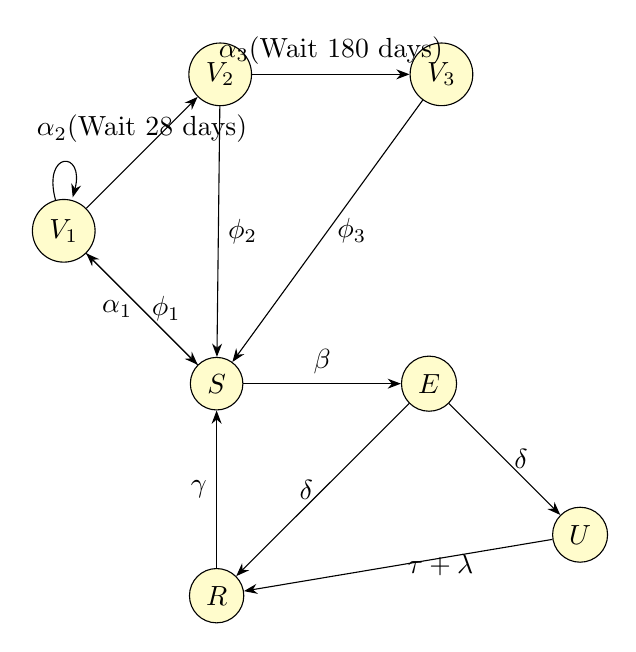
\begin{tikzpicture}[node distance=2cm,>=Stealth]

    % Nodes
    \node[draw, circle, fill=yellow!20] (S) {$S$};
    \node[draw, circle, fill=yellow!20, above left=of S] (V1) {$V_1$};
    \node[draw, circle, fill=yellow!20, above right=of V1] (V2) {$V_2$};
    \node[draw, circle, fill=yellow!20, right=of V2] (V3) {$V_3$};
    \node[draw, circle, fill=yellow!20, right=of S] (E) {$E$};
    \node[draw, circle, fill=yellow!20, below right=of E] (U) {$U$};
    \node[draw, circle, fill=yellow!20, below=of S] (R) {$R$};

    % Arrows
    \draw[->] (S) -- node[above] {$\beta$} (E);
    \draw[->] (E) -- node[right] {$\delta$} (U);
    \draw[->] (E) -- node[left] {$\delta$} (R);
    \draw[->] (U) -- node[right] {$\tau + \lambda$} (R);
    \draw[->] (R) -- node[left] {$\gamma$} (S);
    \draw[->] (S) -- node[left] {$\alpha_1$} (V1);
    \draw[->] (V1) -- node[above] {$\alpha_2$ \\ (Wait 28 days)} (V2);
    \draw[->] (V2) -- node[above] {$\alpha_3$ \\ (Wait 180 days)} (V3);
    \draw[->] (V1) -- node[right] {$\phi_1$} (S);
    \draw[->] (V2) -- node[right] {$\phi_2$} (S);
    \draw[->] (V3) -- node[right] {$\phi_3$} (S);
    \draw[->] (V1) edge[loop above] (V1);

\end{tikzpicture}

\end{document}